% !TeX encoding = UTF-8
% !TeX program = XeLaTeX
% !TeX spellcheck = LaTeX

\documentclass[a4paper]{article}

\usepackage{amsmath,amsfonts,amssymb}
\usepackage{mathrsfs}
\usepackage{bm}
\usepackage{extarrows}
\usepackage{geometry}
\usepackage{ntheorem}
\usepackage{hyperref}
\usepackage[ruled]{algorithm2e}
\usepackage{caption,subcaption}
\usepackage{tikz}

\usetikzlibrary{automata}

\geometry{left=2cm,right=2cm,top=2cm,bottom=2cm}

\def\UrlBreaks{\do\A\do\B\do\C\do\D\do\E\do\F\do\G\do\H\do\I\do\J\do\K\do\L\do\M\do\N\do\O\do\P\do\Q\do\R\do\S\do\T\do\U\do\V\do\W\do\X\do\Y\do\Z\do\[\do\\\do\]\do\^\do\_\do\`\do\a\do\b\do\c\do\d\do\e\do\f\do\g\do\h\do\i\do\j\do\k\do\l\do\m\do\n\do\o\do\p\do\q\do\r\do\s\do\t\do\u\do\v\do\w\do\x\do\y\do\z\do\0\do\1\do\2\do\3\do\4\do\5\do\6\do\7\do\8\do\9\do\.\do\@\do\\\do\/\do\!\do\_\do\|\do\;\do\>\do\]\do\)\do\,\do\?\do\'\do+\do\=\do\#}

\newtheorem{theorem}{Theorem}
\newtheorem{lemma}{Lemma}
\newtheorem{proposition}{Proposition}
\newtheorem{corollary}{Corollary}
\newtheorem{claim}{Claim}
\newtheorem{conjecture}{conjecture}
\newtheorem{definition}{Definition}
\newtheorem{construction}{Construction}
\newtheorem*{proof}{Proof}
\newtheorem*{answer}{Answer}
\newtheorem*{example}{Example}
\newtheorem*{counterexample}{Counterexample}

\newenvironment{exercise}[1]{
	\par
	\noindent\textbf{Exercise #1.}\quad
}{
	\par
	\bigskip
}
\newenvironment{problem}[1]{
	\par
	\noindent\textbf{Problem #1.}\quad
}{
	\par
	\bigskip
}

\DeclareMathAccent{\widehat}{\mathord}{largesymbols}{"62}
\DeclareMathOperator*{\argmax}{\arg\,\max}
\DeclareMathOperator*{\argmin}{\arg\,\min}
\DeclareMathOperator{\E}{\mathbb E}
\DeclareMathOperator{\Var}{\mathrm{Var}}
\DeclareMathOperator{\tr}{\mathrm{tr}}
\DeclareMathOperator{\poly}{\mathrm{poly}}
\newcommand{\abs}[1]{\left| #1 \right|}
\newcommand{\vabs}[1]{\left\| #1 \right\|}
\newcommand{\abra}[1]{\left\langle #1 \right\rangle}
\newcommand{\pbra}[1]{\left( #1 \right)}
\newcommand{\cbra}[1]{\left\{ #1 \right\}}
\newcommand{\sbra}[1]{\left[ #1 \right]}
\newcommand{\floorbra}[1]{\left\lfloor #1 \right\rfloor}
\newcommand{\ceilbra}[1]{\left\lceil #1 \right\rceil}
\newcommand{\bin}{\{0,1\}}
\newcommand{\ZPP}{\mathtt{ZPP}}
\newcommand{\RP}{\mathtt{RP}}
\newcommand{\coRP}{\mathtt{co}\text{-}\mathtt{RP}}
\newcommand{\per}{\text{per}}
\newcommand{\sgn}{\text{sgn}}
\newcommand{\Fbb}{\mathbb{F}}
\newcommand{\Nbb}{\mathbb{N}}
\newcommand{\Rbb}{\mathbb{R}}
\newcommand{\Zbb}{\mathbb{Z}}
\newcommand{\Sset}{\mathbb{S}}
\newcommand{\Fset}{\mathbb{F}}
\newcommand{\Nset}{\mathbb{N}}
\newcommand{\Zset}{\mathbb{Z}}
\newcommand{\Uset}{\mathbb{U}}
\newcommand{\Acal}{\mathcal{A}}
\newcommand{\Bcal}{\mathcal{B}}
\newcommand{\Ccal}{\mathcal{C}}
\newcommand{\Fcal}{\mathcal{F}}
\newcommand{\Gcal}{\mathcal{G}}
\newcommand{\qd}[2]{{\left(\frac{#1}{#2}\right)}}
\newcommand{\dv}{\ |\ }
\newcommand{\mylm}{\xLongrightarrow[lm]{}}
\newcommand{\myrm}{\xLongrightarrow[rm]{}}

\bibliographystyle{plainnat}

\title{Exercise Set --- Chapter $7$}
\date{}

\begin{document}

\maketitle

\noindent\textbf{Notation:}
\begin{itemize}
\item \textit{Pumping length} is \textit{the constant for pumping lemma}.
\item \textit{Ogden length} is \textit{the constant for Ogden's lemma}.
\item $c_t(w)$ counts the number of $t$'s in $w$.
\item $D(w)$ counts the number of \textit{distinguished positions} in $w$.
\item If $w$ is a string, then $w[i]$ stands for the $i$-th character in $w$.
\item $\textit{depth}(T)$ is the depth of tree $T$. (Tree with only one node has depth $0$)
\end{itemize}

\begin{exercise}{7.1.7}
    If the depth of a parse tree is $h$, then $\#\{\text{non-leaf nodes}\}\leqslant
    \sum_{i=0}^{h-1} n^i=\frac{n^h-1}{n-1}.$\par
    Let $T$ be a parse tree of $A$.
    \begin{itemize}
        \item $\textit{depth}(T)\leqslant p$, then
            $\text{derivation steps}=\#\{\text{non-leaf nodes of }T\}\leqslant\frac{n^p-1}{n-1}$.
        \item $\textit{depth}(T)>p$, then there are two identical
            variables along the longest path. Since $A\xLongrightarrow[G]{*}\varepsilon$,
            after replacing the sub parse tree of the upper one with the lower one,
            it is still a valid parse tree.
            Repeat the process until $\textit{depth}(T)\leqslant p$.
    \end{itemize}
    The boundary is tight, considering the following case:
    \small
    \begin{align*}
        S_1 &\to \underbrace{S_2S_2\cdots S_2}_{n}\\
        S_2 &\to \underbrace{S_3S_3\cdots S_3}_{n}\\
        \cdots&\cdots\cdots\cdots\\
        S_{p-1} &\to \underbrace{S_pS_p\cdots S_p}_{n}\\
        S_{p} &\to \varepsilon
    \end{align*}
\end{exercise}

\begin{exercise}{7.1.8} \hspace{0pt}\\
\textbf{a)}
        Assume $A_1,A_2,\cdots,A_k$ are different variables of $G$.
        Let $l_i$ be the length of production body of $A_i$.
        Then $\sum_{i=1}^k l_i=n$. Therefore, the total length of productions after unit elimination is
        no more than
        \begin{align*}
            \sum_{i=1}^k \sum_{\substack{A_i\text{ unit}\\\text{produces }A_j}} l_j
            \leqslant \sum_{i=1}^k \sum_{j=1}^k l_j\leqslant kn=O(n^2).
        \end{align*}
        Since every production $S\to S_1\cdots S_n$ can be converted to CNF using $O(n)$ productions,
        thus
        $$
        \#\{\text{productions in CNF}\}=O(\text{total length in NF})=O(n^2).
        $$\\
\textbf{b)} \textit{W.L.O.G.} assume $n=3m-1$.
    Construct $G=(V,T,P,S)=(\{A_1,A_2,\cdots,A_{m}\},\{a\},P,A_1)$, where $P$ is
    $$
        A_i\to\begin{cases}
            A_{i+1}\dv A_{i}A_{i+1} & i<m\\
            A_1\dv a & i=m
        \end{cases}.
    $$
    Then for any $i,j$, $A_i$ unit produces $A_j$. Thus
    \begin{align*}
        \#\{\text{productions in CNF}\}= \sum_{i=1}^{m} \sum_{j=1}^{m} 1=\frac19 (n+1)^2.
    \end{align*}
\end{exercise}

\begin{exercise}{7.1.10}
    Counterexample: $G=(V,T,P,S)=(\{A\},\{a\},P,A)$, where $P$ is
    \begin{align*}
        A&\to aa
    \end{align*}
\end{exercise}

\begin{exercise}{7.2.1} \hspace{0pt}\\
\textbf{a)} $L=\{a^ib^jc^k|i<j<k\}$
    \begin{proof}
        Assume $L$ is CFL and the pumping length is $n_0$.
        Consider $s=a^{n_0}b^{n_0+1}c^{n_0+2}\in L$, $s=uvwxy,|vwx|\leqslant n_0,|vx|>0,v=c_1^i,x=c_2^j,c_1,c_2\in\{a,b,c\}$.
        \begin{itemize}
            \item $v=a^i,x=a^j,\max\{i,j\}\geqslant 1$, then $uv^2wx^2y=a^{n_0+i+j}b^{n_0+1}c^{n_0+2}\notin L$.
            \item $v=a^i,x=b^j,\max\{i,j\}\geqslant 1$, then $uv^2wx^2y=a^{n_0+i}b^{n_0+1+j}c^{n_0+2}\notin L$.
            \item $v=b^i,x=b^j,\max\{i,j\}\geqslant 1$, then $uv^2wx^2y=a^{n_0}b^{n_0+1+i+j}c^{n_0+2}\notin L$.
            \item $v=b^i,x=c^j,\max\{i,j\}\geqslant 1$, then $uwy=a^{n_0}b^{n_0+1-i}c^{n_0+2-j}\notin L$.
            \item $v=c^i,x=c^j,\max\{i,j\}\geqslant 1$, then $uwy=a^{n_0}b^{n_0+1}c^{n_0+2-i-j}\notin L$.
        \end{itemize}
        A contradiction.
    \end{proof}
\textbf{b)} $L=\{a^nb^nc^i|i\leqslant n\}$
    \begin{proof}
        Assume $L$ is CFL and the pumping length is $n_0$.
        Consider $s=a^{n_0}b^{n_0}c^{n_0}\in L$, $s=uvwxy,|vwx|\leqslant n_0,|vx|>0$.
        Therefore $v=c_1^i,x=c_2^j,c_1,c_2\in\{a,b,c\}$, thus $n_a(uwy)\neq n_b(uwy)$ or $n_a(uwy)\neq n_c(uwy)$,
        which means $uwy\notin L$.
        A contradiction.
    \end{proof}
\textbf{c)} $L=\{0^p|p \text{ is a prime}\}$
    \begin{proof}
        \begin{theorem}\label{sp2}
            Assume $L\subseteq\{0\}^*$, then $L$ is a CFL $\Leftrightarrow$ $L$ is a regular language.
            \begin{proof}
                $\Leftarrow$ Obvious.\par
                $\Rightarrow$ By \textit{Parikh's theorem}, $L=L_1\cup L_2\cup \cdots L_k$, where
                $L_i=\{0^{a_i}0^{m_1b_1+m_2b_2+\cdots+m_{c_i}b_{c_i}}|m_j\in\Nset\}$.
                Since $L_i$ is regular, $L$, which is the union of $L_i$'s,
                is also regular.
            \end{proof}
        \end{theorem}
        Based on Theorem \ref{sp2}, $L$ is CFL iff $L$ is regular.
        Since we know $L$ is not regular, it is not CFL either.
    \end{proof}
\textbf{d)} $L=\{0^i1^j|j=i^2\}$
    \begin{proof}
        Assume $L$ is CFL and the pumping length is $n_0$.
        Consider $s=0^{n_0}1^{n_0^2}\in L$, $s=uvwxy,|vwx|\leqslant n_0,|vx|>0,v=c_1^i,x=c_2^j,c_1,c_2\in\{0,1\}$.
        \begin{itemize}
            \item $v=0^i,x=0^j,\max\{i,j\}\geqslant 1$, then $uv^2wx^2y=0^{n_0+i+j}1^{n_0^2}\notin L$.
            \item $v=1^i,x=1^j,\max\{i,j\}\geqslant 1$, then $uv^2wx^2y=0^{n_0}1^{n_0^2+i+j}\notin L$.
            \item $v=0^i,x=1^j,\max\{i,j\}\geqslant 1$, then $uv^2wx^2y=0^{n_0+i}1^{n_0^2+j}$.
                Since $j\leqslant n_0$, $n_0^2<n_0^2+j<(n_0+1)^2$, thus $uv^2wx^2y\notin L$.
        \end{itemize}
        A contradiction.
    \end{proof}
\textbf{e)} $L=\{a^nb^nc^i|n\leqslant i\leqslant 2n\}$
    \begin{proof}
        Assume $L$ is CFL and the pumping length is $n_0$.
        Consider $s=a^{n_0}b^{n_0}c^{2n_0-1}\in L$, $s=uvwxy,|vwx|\leqslant n_0,|vx|>0,v=c_1^i,x=c_2^j,c_1,c_2\in\{a,b,c\}$.
        \begin{itemize}
            \item $v=a^i,x=a^j,\max\{i,j\}\geqslant 1$, then $uv^2wx^2y=a^{n_0+i+j}b^{n_0}c^{2n_0-1}\notin L$.
            \item $v=a^i,x=b^j,\max\{i,j\}\geqslant 1$, then $uwy=a^{n_0-i}b^{n_0-j}c^{2n_0-1}\notin L$.
            \item $v=b^i,x=b^j,\max\{i,j\}\geqslant 1$, then $uv^2wx^2y=a^{n_0}b^{n_0+i+j}c^{2n_0-1}\notin L$.
            \item $v=b^i,x=c^j,\max\{i,j\}\geqslant 1$, then $uv^2wx^2y=a^{n_0}b^{n_0+i}c^{2n_0-1+j}\notin L$.
            \item $v=c^i,x=c^j,\max\{i,j\}\geqslant 1$, then $uv^2wx^2y=a^{n_0}b^{n_0}c^{2n_0-1+i+j}\notin L$.
        \end{itemize}
        A contradiction.
    \end{proof}
\textbf{f)} $L=\{ww^Rw|w\in\{0,1\}^*\}$
    \begin{proof}
        Assume $L$ is CFL and the pumping length is $n_0$.
        Since $L'=\{1^n0^m1^t0^s\}$ is regular, $\hat{L}:=L\cap L'=\{1^n0^{2n}1^{2n}0^n\}$ is also CFL.
        Consider $s=1^{n_0}0^{2n_0}1^{2n_0}0^{n_0}\in \hat{L}$, $s=uvwxy,|vwx|\leqslant n_0,|vx|>0,v=c_1^i,
        w=c_2^j,c_1,c_2\in\{0,1\}$.
        Label $s$ as $1_a^{n_0}0_a^{2n_0}1_b^{2n_0}0_b^{n_0}$.
        \begin{itemize}
            \item $v=1_a^i,x=1_a^j,\max\{i,j\}\geqslant 1$, then $uv^2wx^2y=1^{n_0+i+j}0^{2n_0}1^{2n_0}0^{n_0}\notin \hat{L}$.
            \item $v=1_a^i,x=0_a^j,\max\{i,j\}\geqslant 1$, then $uv^2wx^2y=1^{n_0+i}0^{2n_0+j}1^{2n_0}0^{n_0}\notin \hat{L}$.
            \item $v=0_a^i,x=0_a^j,\max\{i,j\}\geqslant 1$, then $uv^2wx^2y=1^{n_0}0^{2n_0+i+j}1^{2n_0}0^{n_0}\notin \hat{L}$.
            \item $v=0_a^i,x=1_b^j,\max\{i,j\}\geqslant 1$, then $uv^2wx^2y=1^{n_0}0^{2n_0+i}1^{2n_0+j}0^{n_0}\notin \hat{L}$.
            \item $v=1_b^i,x=1_b^j,\max\{i,j\}\geqslant 1$, then $uv^2wx^2y=1^{n_0}0^{2n_0}1^{2n_0+i+j}0^{n_0}\notin \hat{L}$.
            \item $v=1_b^i,x=0_b^j,\max\{i,j\}\geqslant 1$, then $uv^2wx^2y=1^{n_0}0^{2n_0}1^{2n_0+i}0^{n_0+j}\notin \hat{L}$.
            \item $v=0_b^i,x=0_b^j,\max\{i,j\}\geqslant 1$, then $uv^2wx^2y=1^{n_0}0^{2n_0}1^{2n_0}0^{n_0+i+j}\notin \hat{L}$.
        \end{itemize}
        A contradiction.
    \end{proof}
\end{exercise}

\begin{exercise}{7.2.5} \hspace{0pt}\\
\textbf{a)} $L=\{0^i1^j0^k|j=\max(i,k)\}$.
    \begin{proof}
        Assume $L$ is CFL and the Ogden length is $n_0$.
        Consider $s=0^{n_0}1^{n_0}0^{n_0}\in L$ and mark all $1$'s as distinguished positions, therefore
        $s=uvwxy,D(vwx)\leqslant n_0,D(vx)>0,v=c_1^i,x=c_2^j,c_1,c_2\in\{0,1\}$.
        \begin{itemize}
            \item $v=0^i,x=1^j,j\geqslant 1$, then $uwy=0^{n_0-i}1^{n_0-j}0^{n_0}\notin L$.
            \item $v=1^i,x=1^j,\max\{i,j\}\geqslant 1$, then $uwy=0^{n_0}1^{n_0-i-j}0^{n_0}\notin L$.
            \item $v=1^i,x=0^j,i\geqslant 1$, then $uwy=0^{n_0}1^{n_0-i}0^{n_0-j}\notin L$.
        \end{itemize}
        A contradiction.
    \end{proof}
\textbf{b)} $L=\{a^nb^nc^i|i\neq n\}$.
    \begin{proof}
        Assume $L$ is CFL and the Ogden length is $n_0$.
        Consider $s=a^{n_0}b^{n_0}c^{n_0+n_0!}\in L$ and mark all $a$'s as distinguished positions, therefore
        $s=uvwxy,D(vwx)\leqslant n_0,D(vx)>0,x=c_2^j,c_1,c_2\in\{a,b,c\}$.
        \begin{itemize}
            \item $v=a^i,x=a^j,1\leqslant i+j\leqslant n_0$, then
                $$
                uv^{\frac{n_0!}{i+j}+1}wx^{\frac{n_0!}{i+j}+1}y=0^{n_0+n_0!}1^{n_0}0^{n_0+n_0!}\notin L.
                $$
            \item $v=a^i,x=b^j,1\leqslant i\leqslant n_0$, then
                $$
                uv^{\frac{n_0!}{i}+1}wx^{\frac{n_0!}{i}+1}y=0^{n_0+n_0!}1^{n_0+j\frac{n_0!}{i}}0^{n_0+n_0!}\notin L.
                $$
            \item $v=a^i,x=c^j,i\geqslant 1$, then $uwy=0^{n_0-i}1^{n_0}0^{n_0+n_0!-j}\notin L$.
        \end{itemize}
        A contradiction.
    \end{proof}
\end{exercise}

\begin{exercise}{7.3.2}\hspace{0pt}\\
\textbf{a)}
    $L_1=L(G_1)$. $G_1=(V,T,P,S)=(\{S,S_1,S_2\},\{a,b,c\},P,S)$, where $P$ is
    \begin{align*}
        S &\to S_1S_2\\
        S_1 &\to aS_1bb\dv\varepsilon\\
        S_2 &\to cS_2\dv\varepsilon
    \end{align*}
    $L_2=L(G_2)$. $G_2=(V,T,P,S)=(\{S,S_1,S_2\},\{a,b,c\},P,S)$, where $P$ is
    \begin{align*}
        S &\to S_1S_2\\
        S_1 &\to aS_1\dv\varepsilon\\
        S_2 &\to bS_2cc\dv\varepsilon
    \end{align*}\\
\textbf{b)}
    $L_1\cap L_2$ is not CFL.
    \begin{proof}
        Let $L=L_1\cap L_2=\{a^nb^{2n}c^{4n}|n\geqslant 0\}$.\par
        Assume $L$ is CFL and the Ogden length is $n_0$.
        Consider $s=a^{n_0}b^{2n_0}c^{4n_0}\in L$ and mark all $a$'s as distinguished positions, therefore
        $s=uvwxy,D(vwx)\leqslant n_0,D(vx)>0,x=c_2^j,c_1,c_2\in\{a,b,c\}$.
        \begin{itemize}
            \item $v=a^i,x=a^j,i+j\geqslant 1$, then $uwy=a^{n_0-i-j}b^{2n_0}c^{4n_0}\notin L$.
            \item $v=a^i,x=b^j,i\geqslant 1$, then $uwy=a^{n_0-i}b^{2n_0-j}c^{4n_0}\notin L$.
            \item $v=a^i,x=c^j,i\geqslant 1$, then $uwy=a^{n_0-i}b^{2n_0}c^{4n_0-j}\notin L$.
        \end{itemize}
        A contradiction.
    \end{proof}
\end{exercise}

\begin{exercise}{7.3.3} Assume $L,M$ are CFL.\\
\textbf{a)} $L'=\min(L)=\{w|w\in L,\not\!\exists x,y,y\neq\varepsilon, xy=w\}$.
    \begin{proof}
        Let $L_1=\{0^i1^j2^k|i,j,k\geqslant 1,i\leqslant k\}$ and $L_2=\{0^i1^j2^k|i,j,k\geqslant 1,j\leqslant k\}$.
        Obviously, $L_1,L_2$ are CFL's, therefore $L:=L_1\cup L_2$ is also CFL. However,
        $L'=\{0^i1^j2^k|i,j\geqslant 1,k=\min\{i,j\}\}$ is not CFL.
    \end{proof}
\textbf{b)} $L'=\max(L)=\{w|w\in L,\not\!\exists x\neq\varepsilon,wx\in L\}$.
    \begin{proof}
        Let $L_1=\{0^i1^j2^k|i,j,k\geqslant 1,i\geqslant k$ and $L_2=\{0^i1^j2^k|i,j,k\geqslant 1,j\geqslant k\}$.
        Obviously, $L_1,L_2$ are CFL's, therefore $L:=L_1\cup L_2$ is also CFL. However,
        $L'=\{0^i1^j2^k|i,j\geqslant 1,k=\max\{i,j\}\}$ is not CFL.
    \end{proof}
\textbf{c)} $L'=\textit{half}(L)=\{w|\exists x,|w|=|x|,wx\in L\}$.
    \begin{proof}
        Consider $L=\{0^i1^j2^j3^{3i}|i,j\geqslant 0\}$. Firstly, $L$ is a CFL.
        Let $G=(V,T,P,S)=(\{S,S_1\},\{0,1,2,3\},P,S)$, where $P$ is
        \begin{align*}
            S &\to 0S333\dv S_1\\
            S_1 &\to 1S_12\dv \varepsilon
        \end{align*}
        Thus $L(G)=L$.\par
        Secondly,
        $$
        L_{1/2}=\{0^i1^j2^i|j\geqslant i\}\cup\{0^i1^j2^j3^{i-j}|i>j\}
        $$
        is not a CFL. \par
        Assume $L_{1/2}$ is a CFL and $n_0$ be its pumping length. Consider
        $s=0^{n_0}1^{n_0}2^{n_0}\in L_{1/2}$. Then $s=uvwxy, |vx|>0, |vwx|\leqslant n_0,v=c_1^i,x=c_2^j,c_1,c_2\in\{0,1,2\}$.
        \begin{itemize}
            \item $v=0^i,x=0^j,i+j>0$, then $uv^2wx^2y=0^{n_0+i+j}1^{n_0}2^{n_0}\notin L_{1/2}$.
            \item $v=0^i,x=1^j,\max\{i,j\}>0$, then $uwy=0^{n_0-i}1^{n_0-j}2^{n_0}\notin L_{1/2}$.
            \item $v=1^i,x=1^j,i+j>0$, then $uwy=0^{n_0}1^{n_0-i-j}2^{n_0}\notin L_{1/2}$.
            \item $v=1^i,x=2^j,\max\{i,j\}>0$, then $uwy=0^{n_0}1^{n_0-j}2^{n_0-i}\notin L_{1/2}$.
            \item $v=2^i,x=2^j,i+j>0$, then $uv^2wx^2y=0^{n_0}1^{n_0}2^{n_0+i+j}\notin L_{1/2}$.
        \end{itemize}
        A contradiction.
    \end{proof}
\textbf{d)} $L'=\textit{alt}(L,M)=\{a_1b_1a_2b_2\cdots a_nb_n|a_1a_2\cdots a_n\in L,b_1b_2\cdots b_n\in M\}$.
    \begin{proof}
        Let $L=\{0^n1^{2n}|n\in\Nset\}$ and $M=\{2^{2n}3^n|n\in\Nset\}$. It is obvious that $L,M$ are CFL's.
        However, $L'=\{(02)^n(12)^n(13)^n|n\in\Nset\}$ is not CFL,
    \end{proof}
\end{exercise}

\begin{exercise}{7.3.4} \hspace{0pt}\\
\textbf{a)} $\textit{shuffle}(00,111)=\{00111,01011,01101,01110,10011,10101,10110,11001,11010,11100\}$.\\
\textbf{b)} $\textit{shuffle}(L_1,L_2)=\{0^nw|w\in\{0,1\}^*,c_1(w)=n\}$.\\
\textbf{c)}
        Assume DFA $A=(Q,\Sigma,\delta,q_0,F)$ accepts $L$ and DFA $B=(Q',\Sigma',\delta',q'_0,F')$ accepts $R$.
        Construct NFA $C=(Q\times Q',\Sigma\cup\Sigma',\hat{\delta},(q_0,q'_0),F\times F')$, where
        $$
        \hat{\delta}\Big((q,q'),c\Big)=\left\{\Big(\delta(q,c),q'\Big),\Big(q,\delta(q',c)\Big)\right\}.
        $$
        Therefore $C$ accepts $\textit{shuffle}(L,R)$.\\
\textbf{d)}
        Assume PDA $A=(Q,\Sigma,\Gamma,\delta,q_0,Z_0,F)$ accepts $L$ and DFA $B=(Q',\Sigma',\delta',q'_0,F')$ accepts $R$.
        Construct PDA $C=(Q\times Q',\Sigma\cup\Sigma',\Gamma,\hat{\delta},(q_0,q'_0),Z_0,F\times F')$, where
        $$
        \hat{\delta}\Big((q,q'),c,X\Big)=\begin{cases}
            \left\{\Big(\big(q,\delta'(q',c)\big),X\Big)\right\}\cup\left\{\Big((p,q'),\alpha\Big)\middle|
            (p,\alpha)\in\delta(q,c,X)\right\} & c\neq\varepsilon\\
            \left\{\Big((p,q'),\alpha\Big)\middle| (p,\alpha)\in\delta(q,c,X)\right\} & c=\varepsilon
        \end{cases}.
        $$
        Therefore $C$ accepts $\textit{shuffle}(L,R)$.\\
\textbf{e)}
        Let $L_1=\{0^n1^n|n\in\Nset\}$ and $L_2=\{2^n3^n|n\in\Nset\}$, both of which are CFL's.
        Let $\widehat{L}=\{0^a2^b1^c3^d|a,b,c,d\in\Nset\}$, which is regular.\par
        Assume $L:=\textit{shuffle}(L_1,L_2)$ is CFL, then $L\cap\widehat{L}=\{0^n2^m1^n3^m|n,m\in\Nset\}$ is CFL.
        A contradiction.
\end{exercise}

\begin{exercise}{7.3.5} \hspace{0pt}\\
\textbf{a)} $L=\{(01)^n|n\geqslant 0\}$ is regular,
but $\textit{perm}(L)=\{w\in\{0,1\}^*|c_0(w)=c_1(w)\}$ is not regular.\\
\textbf{b)} $L=\{(012)^n|n\geqslant 0\}$ is regular,
but $\textit{perm}(L)=\{w\in\{0,1,2\}^*|c_0(w)=c_1(w)=c_2(w)\}$ is not a CFL.\\
\textbf{c)}
        Assume $L\subseteq\{0,1\}^*$ is regular and DFA $M=(Q,\Sigma,\delta,q_0,F),\Sigma=\{0,1\}$ accepts it.
        Construct PDA $N$ for $\textit{perm}(L)$ based on $M$
        \begin{itemize}
        \item Add $q_0'$ as new initial state in $N$
            \begin{center}
            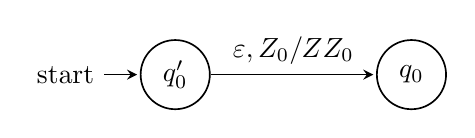
\begin{tikzpicture}[shorten >=1pt,->,>=stealth,semithick,node distance=3cm,auto,align=center]
                \node[state,initial] (p) {$q_0'$};
                \node[state] (q) [right of=p] {$q_0$};
                \path[->] (p) edge node {$\varepsilon,Z_0/ZZ_0$} (q);
            \end{tikzpicture}
            \end{center}
        \item Add $q_f$ as new accepting state in $N$: for every $q_i\in F$
            \begin{center}
            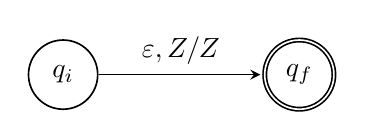
\begin{tikzpicture}[shorten >=1pt,->,>=stealth,semithick,node distance=3cm,auto,align=center]
                \node[state] (p) {$q_i$};
                \node[state,accepting] (q) [right of=p] {$q_f$};
                \path[->] (p) edge node {$\varepsilon,Z/Z$} (q);
            \end{tikzpicture}
            \end{center}
        \item Consider every edge in $M$: for every $q_i,q_j\in Q$, if
            \begin{center}
            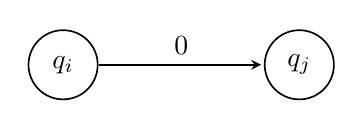
\begin{tikzpicture}[shorten >=1pt,->,>=stealth,semithick,node distance=3cm,auto,align=center]
                \node[state] (p) {$q_i$};
                \node[state] (q) [right of=p] {$q_j$};
                \path[->] (p) edge node {$0$} (q);
            \end{tikzpicture}
            \end{center}
            then construct three edges in $N$, where $*\in\Gamma$;
            \begin{center}
            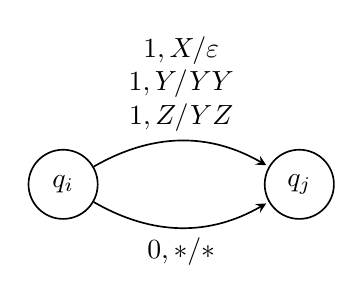
\begin{tikzpicture}[shorten >=1pt,->,>=stealth,semithick,node distance=3cm,auto,align=center]
                \node[state] (p) {$q_i$};
                \node[state] (q) [right of=p] {$q_j$};
                \path[->] (p) edge[bend right] node[below] {$0,*/*$} (q)
                              edge[bend left] node[above] {$1,X/\varepsilon$\\$1,Y/YY$\\$1,Z/YZ$} (q);
            \end{tikzpicture}
            \end{center}
            for every $q_i,q_j\in Q$, if
            \begin{center}
            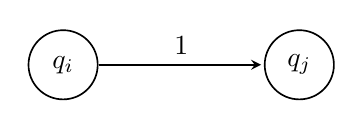
\begin{tikzpicture}[shorten >=1pt,->,>=stealth,semithick,node distance=3cm,auto,align=center]
                \node[state] (p) {$q_i$};
                \node[state] (q) [right of=p] {$q_j$};
                \path[->] (p) edge node {$1$} (q);
            \end{tikzpicture}
            \end{center}
            then construct three edges in $N$, where $*\in\Gamma$;
            \begin{center}
            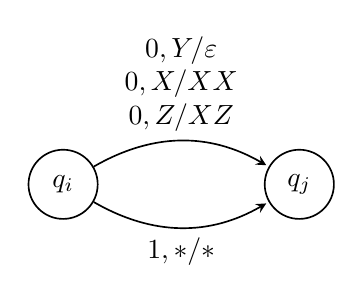
\begin{tikzpicture}[shorten >=1pt,->,>=stealth,semithick,node distance=3cm,auto,align=center]
                \node[state] (p) {$q_i$};
                \node[state] (q) [right of=p] {$q_j$};
                \path[->] (p) edge[bend right] node[below] {$1,*/*$} (q)
                              edge[bend left] node[above] {$0,Y/\varepsilon$\\$0,X/XX$\\$0,Z/XZ$} (q);
            \end{tikzpicture}
            \end{center}
        \end{itemize}
        The key idea here is that if $w\in L,w'\in\textit{perm}(w)$, then $\#\{i|w[i]=0,w'[i]=1\}=\#\{i|w[i]=1,w'[i]=0\}$,
        so use the stack to simulate the equality.
\end{exercise}

\begin{exercise}{7.4.4} 
        Assume $G$ is a CNF grammar; $w\in L(G)$ and $|w|=n$. Let $T$ be a parse tree for
        $w$ and $m=\#\{\text{interior nodes}\}$. Since it is CNF, $T$ is a binary tree
        and the number of interior nodes with degree $1$ is $n$, same as $\#\{\text{leaf nodes}\}$.
        Therefore there are $m-n$ interior nodes with degree $2$.
        As a result,
        $$
        m+n-1=\#\{\text{edges}\}=2(m-n)+n,
        $$
        which gives $m=2n-1$.
\end{exercise}

\end{document}
